\documentclass[aps, prb, twocolumn, a4paper, floatfix, reprint]{revtex4-2}
\usepackage[%
    margin=10mm,% ако не си принтира 10мм не изглежда грозно, а може да събереш повече текст
    % showframe=true,%
    ]{geometry}
\usepackage[T1,T2A]{fontenc}
\usepackage[utf8]{inputenc}
\usepackage[main=bulgarian, english]{babel}
\usepackage{float}
\AtBeginDocument{\selectlanguage{bulgarian}}
\newcommand{\degree}{^{\circ}}
\usepackage{amsmath}
\usepackage{graphics}
\usepackage{graphicx}
\graphicspath{{.}}
\newcommand{\abs}[1]{\lvert#1\rvert}
\let\phi\varphi
\usepackage{booktabs} % от тук се използва само \midrule може и без него 
%\usepackage{adjustbox} % това може да се използва, за да „смаляваш“ широки таблици
%\usepackage{tabularx} % дефинира колона X в среда tabularx която добавя празно място така че цялата таблица да запълни определена ширина
\usepackage{dcolumn}
\newcolumntype{d}[1]{D{.}{.}{#1}}
\usepackage[unicode=true,pdfusetitle]{hyperref}


\makeatletter
\renewcommand{\Dated@name}{}%
\makeatother



\begin{document}
\title{Реверсионно махало}
\author{Васил Николов}
\noaffiliation
\date{03.01.2022}
\maketitle

\section{Цел на упражнението}
Да се изследва поведението на реверсионно махало и да се измери земното ускорение $g$.

\section{Експериментална установка}
Реверсионното махало е метална пръчка с тежести, които могат да се плъзгат по пръчката, и две възможни точки на окачване в двата края на пръчката. Едната тежест се фиксира в единия край, а другата се плъзга по пръта, и се измерват периодите на махалото спрямо двете точки на окачване като функция на разстоянието между тежестите. Теоретично може да се изведе че ако за дадено разстояние между тежестите двата периода $T$ и $T'$ съвпадат, то
\begin{gather*} 
    T = 2\pi \sqrt{\frac{l}{g}} \\
    g = \frac{4\pi^2 l}{T^2} \label{eq:1} \tag{1}
\end{gather*}
където $l$ е разстоянието между двете точки на окачване. По този начин може много точно да се определи земното ускорение.  

\section{Теоретична обосновка}
Плъзгането на едната тежест променя инерчният момент на махалото, и затова то има различни периоди в зависимост от разстоянието между тежестите. От теоремата на Щайнер се извежда уравнение \eqref{eq:1}, и по него се пресмята земното ускорение. 

\section{Експериментални данни и резултати}

\begin{figure}[H]
    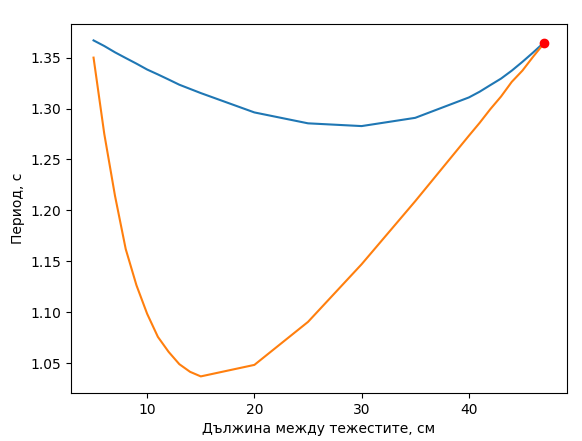
\includegraphics[width=0.9\columnwidth, keepaspectratio=true]{fig_1.png}
\end{figure}

На фигурата се вижда зависимостта на двата периода на махалото като функция на разстоянието между тежестите. Червената точка е индикатор за това къде графиките се пресичат. От точни измервания по графиката се намира координатата на пресечната точка, която в случая отговаря на период $T=(1.3653 \pm 0.001)s$. Разстоянието между точките на окачване е $l=(46.314 \pm 0.002)cm$. Използвайки \eqref{eq:1} крайната стойност за земното ускорение е 
\begin{equation*}
    g = 9.809 \pm 0.02 ms^{-2} 
\end{equation*} 
Тази стойност на земното ускорение е в съгласие в общоприетата стойност $g=9.81 ms^{-2}$.


\end{document}